\chapter{O Método de Traçamento de Raios}

    \label{cap:RT}

    \section{O Funcionamento e a Finalidade}
    
        O traçamento de raios é uma técnica que, basicamente, consiste em modelar a propagação de ondas através de um \textit{meio} elástico utilizando ferramentas chamadas \textit{raios}. 
        
        No caso do traçamento tratado nesse trabalho, consideraremos um modelo de propagação de ondas sísmicas em uma geologia acamadada. Esses raios são emitidos por uma fonte na superfície do meio e traçados, de acordo com uma lei matemática (a ser mostrada na Seção \ref{raySec}), até que alguma camada do meio seja encontrada. Nesse momento, aplica-se a lei de Snell sobre o raio de acordo com a propriedade da camada (se ela é refletora ou transmissora) e inicia-se novamente o traçamento, como se a última camada encontrada fosse a nova fonte. Isso ocorre até que a superfície seja alcançada. Na superfície podem existir receptores que podem ser atingidos pelos raios traçados \cite{notasAulas2017}.
        
        Podemos ter alguma ideia do procedimento descrito acima com a ajuda da Figura \ref{fig:rayTracing}. A fonte emite os raios que atravessam as camadas transmissoras até alcançar a camada refletora previamente definida. A partir daí, os raios sobem até os receptores.
        
        \begin{figure}[H]
            \centering
            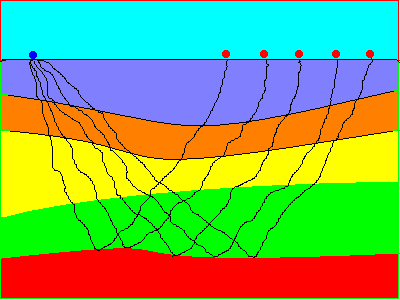
\includegraphics[scale=.8]{imagens/ilustracoes/rayTracing.png}
            
            \hrulefill
            \caption{Imagem meramente ilustrativa sobre o traçamento de raios. O ponto azul representa uma fonte e os pontos vermelhos, receptores. As camadas da subsuperfície são ilustradas pelas cores lilás, laranja, amarelo, verde e vermelho, respectivamente, sendo essa última a camada refletora dos raios e as demais, transmissoras. As linhas pretas que ligam a fonte aos receptores são os raios.}
            \hrulefill
            \label{fig:rayTracing}
        \end{figure}
        
        Existem vários outros tipos de traçamento de raios, podendo-se ter todos os raios emitidos pela fonte refletidos em um único ponto de alguma camada do meio ou todos os raios emitidos refletindo para um único receptor. No geral, todos esses tipos de traçamento de raios visam possibilitar a análise da estrutura de um determinado meio usando-se as propriedades da propagação de ondas para isso \cite{notasAulas2017}.
    
    \section{O Meio}
    
        O meio a ser vasculhado pelo traçamento de raios pode ser formado ou não por camadas. Para esse trabalho, assumimos um meio formado por camadas, sendo essas dispostas uma por cima da outra e com a condição de que uma camada pode ter contato apenas com, no máximo, duas outras. Além disso, consideramos a atmosfera encontrada acima da primeira camada como uma dessas também. Esse meio é uma adaptação do que seria um meio \textbf{acamadado} no ramo da sismologia \cite{notasAulas2017}.
        
        Cada uma das camadas do meio possui como propriedades principais sua espessura, os formatos e posições de suas interfaces (que separam uma camada de outra) e a sua velocidade sísmica, que é ``a taxa pela qual uma onda sísmica viaja através de um meio, que é, a distância dividida pelo tempo de trânsito'' \cite{OilfieldGlossary:seismicVelocity}, sendo o tempo de trânsito a ``duração da passagem de um sinal a partir de uma fonte através da Terra e voltando para um receptor'' \cite{OilfieldGlossary:travelTime}.
        
        Na sismologia, a determinação dessas propriedades das camadas é importante para que se possa cogitar sobre os materiais que formam cada camada e, dependendo da aplicação do método, como esses materiais poderiam ser alcançados fisicamente.
    
    \section{O Raio}
    
        \label{raySec}
        
            Modelar campos de ondas computacionalmente tem um alto custo. Para contornar esse problema, utilizamos a teoria dos raios ao nosso favor. Um raio é como uma parte infinitesimal de uma frente de onda ao longo do tempo, sendo também perpendicular a esta. Um conjunto de raios que simulam partes da mesma frente de onda tomam o formato dela no decorrer do tempo, o que seria possível observar se a propagação da frente de onda fosse simulada por completo. Utilizando apenas pequenas partes (raios) de um domínio muito maior (frente de onda), o traçamento de raios consegue superar a simulação completa no que tange ao custo computacional.
    
            Como dito, o raio simula uma pequena parte de uma frente de onda \textbf{ao longo do tempo}. Ora, mas o que significa a expressão explicitada? Quer dizer que cada ponto do corpo do raio é a posição da parte infinitesimal da frente de onda representada no tempo. Para tentar entender essa questão mais facilmente, veja a Figura \ref{fig:ray&WavePropagation}
            \begin{figure}[H]
                \centering
                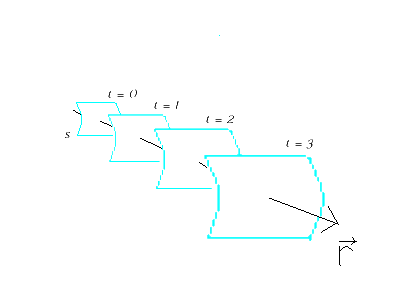
\includegraphics[scale=.8]{imagens/ilustracoes/ray.png}
                \caption{Propagação de uma parte infinitesimal $s$ de uma frente de onda, ao longo do tempo $t$, na direção de um vetor $\vec{r}$. A trajetória do vetor $\vec{r}$ ao longo do tempo forma o raio.}
                \label{fig:ray&WavePropagation}
            \end{figure}
            Imagine que o vetor $\vec{r}$ é sempre perpendicular à frente de onda e a segue. Se traçássemos os pontos de sua trajetória ao longo do tempo, teríamos então um raio e, por ele, a forma como a frente de onda propagou no decorrer do tempo.
            
            \subsection{Uma Brevíssima Visão Sobre a Teoria dos Raios}
            
                A teoria dos raios possui se baseia numa teoria matemática muito complexa e densa, em um nível que foge ao escopo desse trabalho. Por isso, explicaremos do que se trata essa teoria da forma mais básica possível.
                
                Assumamos ondas de alta frequência. Sabemos que a equação da onda é algo como 
                \begin{equation}
                    \label{eqOndaRaySec}
                    \nabla^2u(\vec{x}, t) - \dfrac{1}{\alpha^2}\dfrac{\partial^2u(\vec{x}, t)}{\partial t^2} = 0
                \end{equation}
                onde $\nabla^2$ é o operador laplaciano, que representa
                \begin{equation}
                    \nabla^2 = \dfrac{\partial^2}{\partial x^2} + \dfrac{\partial^2}{\partial y^2}
                \end{equation}
                para o caso de duas dimensões espaciais e $\vec{x}$ é o vetor posição em $x$ e $y$. Então, se assumirmos uma solução harmônica como
                \begin{equation}
                    u(\vec{x}, t) = A(\vec{x})e^{-i\omega(T(\vec{x}) + t)}
                \end{equation}
                na qual $\omega$ é a frequência da onda, $A(\vec{x})$ é a amplitude de uma determinada posição $(x, y)$ da onda e $T(\vec{x}) = c$ é uma frente de onda (o $\nabla T$ define o \textit{raypath}, ou seja, uma linha, sempre perpendicular à frente de onda no caso dos meios isotrópicos, que define as direções que a propagação da onda assumiu \cite{OilfieldGlossary:raypath}), e, usando as derivadas da solução, realizarmos as devidas substituições e manipulações na equação da onda \ref{eqOndaRaySec} teremos que a equação resultante pode ser separada em suas partes real e imaginária \cite{RawlinsonSlide06_RayTheory}.
                
                A parte real,
                \begin{equation}
                    \nabla^2A - \omega^2A|\nabla T|^2 = \dfrac{-A\omega^2}{\alpha^2}
                \end{equation}
                que, ao ser dividida por $A\omega^2$ e levando-se em conta a hipótese de ondas de alta frequência ($\omega \rightarrow \infty$), leva à \textbf{equação iconal}
                \begin{equation}
                    \label{eikonalEquation}
                    |\nabla T| = \dfrac{1}{\alpha^2}
                \end{equation}
                que ``descreve a propagação cinemática de ondas de alta frequência'' \cite{RawlinsonSlide06_RayTheory} (tradução nossa). O lado direito dessa equação, $\dfrac{1}{\alpha^2}$, é chamado \textbf{vagarosidade} \cite{RawlinsonSlide06_RayTheory}. Já a parte imaginária,
                \begin{equation}
                    2\omega\nabla A\cdot\nabla T + \omega A\nabla^2T = 0
                \end{equation}
                ao ser dividida por $\omega$, leva a \textbf{equação de transporte},
                \begin{equation}
                    2\nabla A\cdot\nabla T + A\nabla^2T = 0
                \end{equation}
                que ``pode ser usada para computar a amplitude das ondas que estão propagando'' \cite{RawlinsonSlide06_RayTheory}.
                
                Da equação iconal (\ref{eikonalEquation}), utilizando o processo aplicado em \cite{Miqueles2006}, obtemos o sistema de equações 
                \begin{align}
                    \dfrac{d\vec{x}}{dT} &= v(x)^2\vec{p}\\
                    \dfrac{d\vec{p}}{dT} &= \dfrac{1}{v(x)}\nabla v(\vec{x})
                \end{align}
                nas quais, $\vec{p}$ é chamado \textbf{vetor vagarosidade}. A solução desse sistema é algo no formato $(\vec{x}, \vec{p})$, sendo $\vec{x}$, quando o problema é resolvido computacionalmente, um \textit{array} de alguns dos pontos pelos quais o raio passou. Já $\vec{p}$ é um \textit{array} de algumas direções assumidas pelo raio ao longo do traçamento \cite{Miqueles2006}. Digo algumas porque a solução analítica possui infinitos pontos e infinitas direções durante o traçamento, mas isso não ocorre computacionalmente.